\section{Felhasználói fiók}
\rhead{Felhasználói fiók}

\subsection{Regisztráció}
Az Archytex alkalmazásban a szolgáltatások használatához felhasználói fiók létrehozására van szükség. Ez a honlapon a \emph{/register} útvonalon vagy a bejelentkezés oldalon a \emph{Csatlakozz az Archytex-hez} link használatával elérhető regisztrációs lapon tehető meg.

\begin{samepage}
  \noindent Regisztrációhoz szükséges adatok:
  \begin{itemize}
    \item Felhasználónév
    \item E-mail cím
    \item Jelszó
  \end{itemize}
\end{samepage}

\begin{figure}[H]
  \centering
  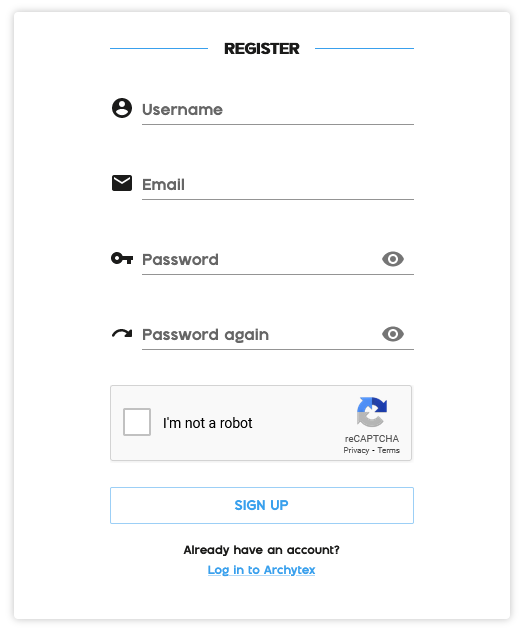
\includegraphics[scale=.5]{parts/user-documentation/account/images/register.png}
  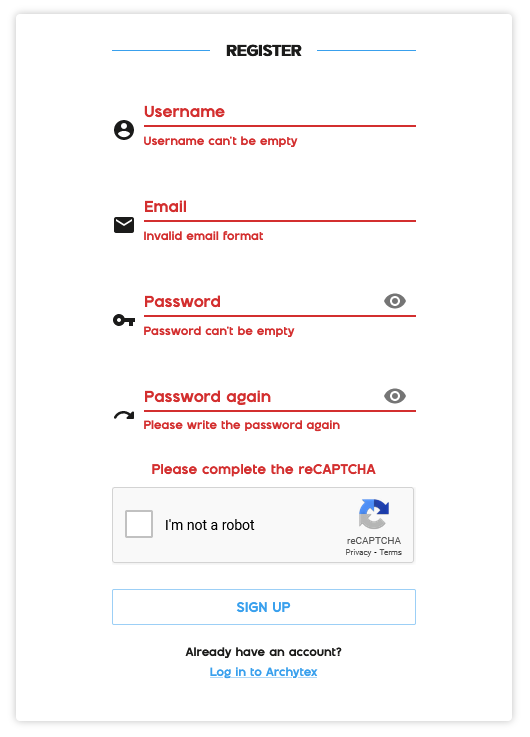
\includegraphics[scale=.5]{parts/user-documentation/account/images/register-errors.png}
  \caption{A regisztrációs űrlap és a hibaüzenetek kijelzése}
\end{figure}

A regisztrációs és a bejelentkezési űrlapon is történik hibakezelés, így nem adható meg hibás adat. Új fiók létrehozása után a megadott e-mail címre küldött levélben található linkkel erősíthető meg a regisztráció.

\subsection{Bejelentkezés}
A bejelentkezési képernyő a honlapon a \emph{/login} útvonalon vagy asztali nézeten a navigációs csík jobb oldalán található \emph{Bejelentkezés} gombbal, telefonos nézeten pedig a hamburger ikonnal kinyitható navigációs menüben található \emph{Bejelentkezés} gombbal érhető el. Bejelentkezés csak a már regisztrált és a regisztrációt megerősített fiókokkal lehetséges.

\begin{figure}[H]
  \centering
  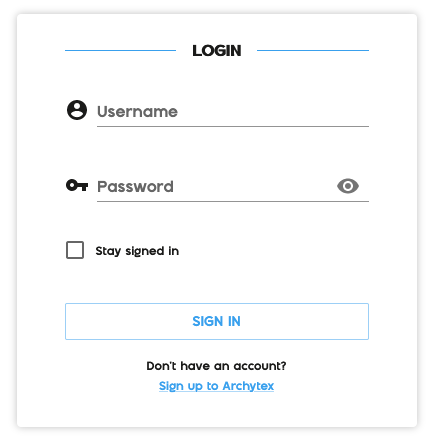
\includegraphics[scale=.6]{parts/user-documentation/account/images/login.png}
  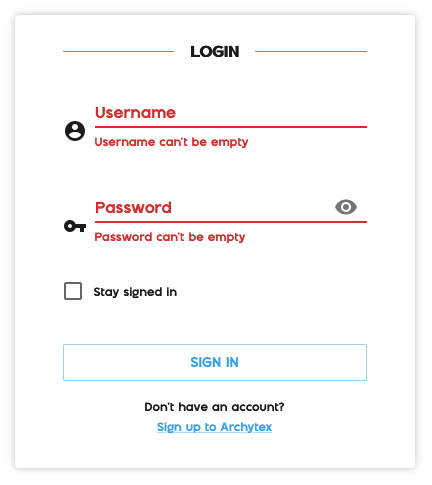
\includegraphics[scale=.6]{parts/user-documentation/account/images/login-errors.png}
  \caption{A bejelentkezési űrlap és a hibaüzenetek kijelzése}
\end{figure}

\subsection{Felhasználók számára elérhető funkciók}
Bejelentkezés után a felhasználó számára elérhetővé válnak az Archytex által nyújtott szolgáltatások. Megjelenik a navigációs csíkon a vezérlőpult; itt lehetséges új projektek létrehozása, valamint a projektek megnyitása a szerkesztőben. Ugyanúgy a navigációs csíkon található a jobb oldalon a profil ikon, amelyre kattintva egy menü nyitható meg. Ezen menüben található a \emph{Beállítások} és a \emph{Kijelentkezés} gomb.

A szerkesztőben készített jelenetek elmenthetőek a fejlécben található \emph{Mentés} gombbal. A projekt következő megnyitásakor az elmentett állapot fog megjelenni. Emellett lehetőség van az elkészített jelenetek renderelésére. Egy projekthez tartozó renderek a vezérlőpulton a projekt lenyitása után tekinthetőek meg.